\documentclass[a4paper,english]{article}
%\usepackage[T1]{fontenc}		% la font bien
\usepackage[utf8]{inputenc}		% les accents
\usepackage[french]{babel}		% la langue
\usepackage{amsmath,amssymb}	% math
\usepackage{graphicx,color,import,float,subcaption}  % graph
\usepackage[usenames,dvipsnames]{xcolor}
\usepackage[margin=2cm]{geometry} % marges
\usepackage{multicol,multirow}	% tables
\usepackage{todonotes}			% penses-bêtes
\usepackage{wrapfig}			% figures sur le côté
\usepackage{hyperref}			% liens vers les figures et formules
\usepackage{lipsum, comment}

\renewcommand{\thesubfigure}{\roman{subfigure}} 
% Numérotation romaine des sous-figures pour éviter collision avec légende

\begin{document}

\title{Potentiel chimique d'un gaz de Bosons}
\author{Mario Geiger}
\date{\today}
\maketitle

\section{Introduction}

\begin{figure}
	\centering
	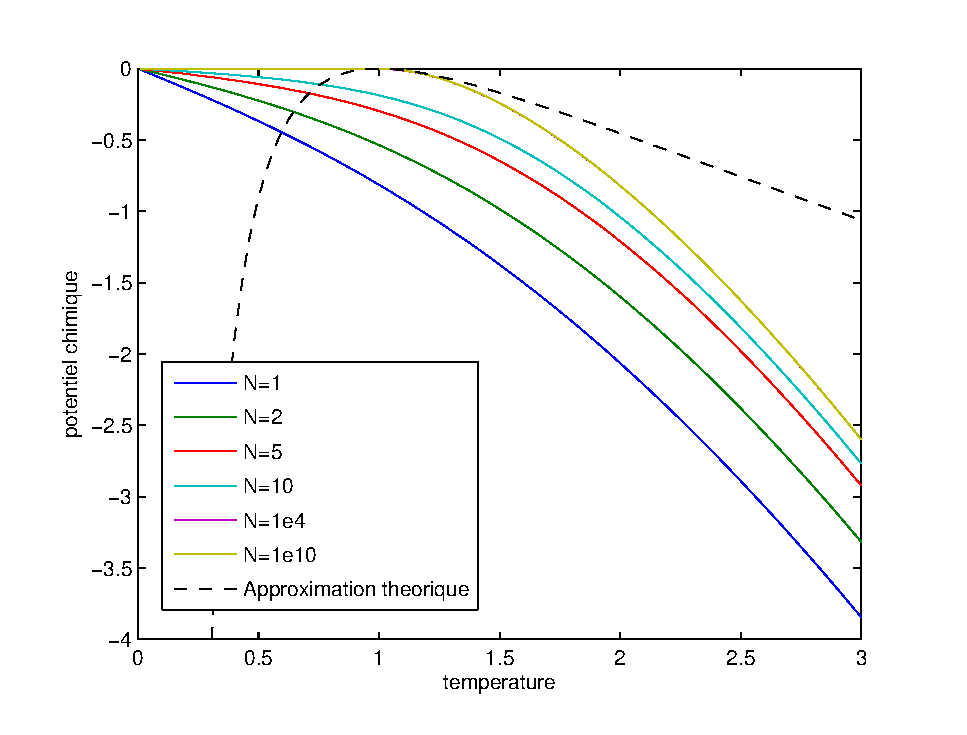
\includegraphics{untitled.eps}
	\caption{Le potentiel chimique en fonction du nombre de Bosons.}
\end{figure}


\end{document}
